%%%%%%%%%%%%%%%%%%%%%%%%%%%%%%%%%%%%%%%%%%%%%%%%%%%%%%%%%%%%%%%%%%%%%
%%                                                                 %%
%% Please do not use \input{...} to include other tex files.       %%
%% Submit your LaTeX manuscript as one .tex document.              %%
%%                                                                 %%
%% All additional figures and files should be attached             %%
%% separately and not embedded in the \TeX\ document itself.       %%
%%                                                                 %%
%%%%%%%%%%%%%%%%%%%%%%%%%%%%%%%%%%%%%%%%%%%%%%%%%%%%%%%%%%%%%%%%%%%%%

\documentclass[pdflatex,sn-mathphys]{sn-jnl}% Basic Springer Nature Reference Style/Chemistry Reference Style

%%%% Standard Packages and macros (don't forget to paste the macros in
%%%% the main at the end of the writing).
\usepackage{todonotes}
\usepackage{lstvhdl, lstautogobble, lstpseudocoq}
\usepackage{enumitem}
\usepackage{ebproof}
\ebproofset{left label template=\fontsize{9}{11}\selectfont\inserttext}
\ebproofset{right label template=\fontsize{7}{10}\selectfont\inserttext}

%%%%%%%%%%%%%%%%%%%%%%%%%%%%%%%%%%%%%%
%%%%%%% Misc. macros and defs. %%%%%%%
%%%%%%%%%%%%%%%%%%%%%%%%%%%%%%%%%%%%%%

% Macro definitions.

\def\bbook{\textsf{B}-Book}
\def\bmth{\textsf{B}}
\def\cakeml{\textsf{CakeML}}
\def\cnrs{\textsf{CNRS}}
\def\coq{\textsf{Coq}}
\def\java{\textsf{Java}}
\def\hilecop{\textsf{HILECOP}}
\def\inria{\textsf{Inria}}
\def\isahol{\textsf{Isabelle/HOL}}
\def\isa{\textsf{Isabelle}}
\def\hol{\textsf{HOL}}
\def\ccert{\textsf{CompCert}}
\def\lirmm{\textsf{LIRMM}}
\def\lustre{\textsf{Lustre}}
\def\nasa{\textsf{NASA}}
\def\um{\textsf{Universit\'e de Montpellier}}
\def\neurin{\textsf{NEURINNOV}}
\def\uml{\textsf{UML}}
\def\vhdl{\textsf{VHDL}}
\def\hvhdl{$\mathcal{H}$-\textsf{VHDL}}
\def\lwidth{\dimexpr\linewidth-2\fboxsep-2\fboxrule}
\def\ocaml{\textsf{OCaml}}

% Circled text

\newcommand\circled[1]{\tikz[baseline=(char.base)]{\node (char) [draw, circle,
    inner sep=1pt] {\small #1};}}

% MAth symbols

\newcommand\srarrow[2]{%
  \mathrel{%
    \begin{tikzpicture}[%
      baseline={(current bounding box.south)}
      ]
      \node[%
      ,inner sep=1ex
      ,align=center
      ] (tmp) {#2 $#1$};
      \path[%
      ,draw,<-,] 
      ($(tmp.south east)+(0,2pt)$) -- ($(tmp.south west)+(3pt,2pt)$);
    \end{tikzpicture}
  }
}


%%% Local Variables:
%%% mode: latex
%%% TeX-master: "main"
%%% End:


%%%%

\jyear{2022}%

%% as per the requirement new theorem styles can be included as shown below
\theoremstyle{thmstyleone}%
\newtheorem{theorem}{Theorem}%  meant for continuous numbers
%%\newtheorem{theorem}{Theorem}[section]% meant for sectionwise numbers
%% optional argument [theorem] produces theorem numbering sequence instead of independent numbers for Proposition
\newtheorem{proposition}[theorem]{Proposition}% 
%%\newtheorem{proposition}{Proposition}% to get separate numbers for theorem and proposition etc.

\theoremstyle{thmstyletwo}%
\newtheorem{example}{Example}%
\newtheorem{remark}{Remark}%

\theoremstyle{thmstylethree}%
\newtheorem{definition}{Definition}%

\raggedbottom
%%\unnumbered% uncomment this for unnumbered level heads

\begin{document}

\title[Formal verification of the \hilecop{} methodology]{Formal verification of a methodology for the design and
  production of safety-critical digital systems}

%%=============================================================%%
%% Prefix	-> \pfx{Dr}
%% GivenName	-> \fnm{Joergen W.}
%% Particle	-> \spfx{van der} -> surname prefix
%% FamilyName	-> \sur{Ploeg}
%% Suffix	-> \sfx{IV}
%% NatureName	-> \tanm{Poet Laureate} -> Title after name
%% Degrees	-> \dgr{MSc, PhD}
%% \author*[1,2]{\pfx{Dr} \fnm{Joergen W.} \spfx{van der} \sur{Ploeg} \sfx{IV} \tanm{Poet Laureate} 
%%                 \dgr{MSc, PhD}}\email{iauthor@gmail.com}
%%=============================================================%%

\author*[1]{\fnm{Vincent} \sur{Iampietro}}
\author[1]{\fnm{David} \sur{Delahaye}}
\author[1,2]{\fnm{David} \sur{Andreu}}

\email{Firstname.Lastname@lirmm.fr}
\email{David.Andreu@neurinnov.com}

\affil*[1]{\orgname{\lirmm, \um, \cnrs},
  \city{Montpellier}, \country{France}}

\affil[2]{\orgname{\neurin}, \city{Montpellier}, \country{France}}

\abstract{}

\keywords{}

\maketitle

\listoftodos

\include{intro}
\section{Models of digital systems in \hilecop{}}
\label{sec:hilecop-models}

Let us introduce the input formalism of \hilecop{}'s model-to-text
transformation: Synchronously executed, extended, generalized,
Interpreted Time Petri Nets with priorities (SITPNs). The
formalization of the SITPN structure and semantics is mainly the
result of two Ph.D. theses \cite{Leroux2014,Merzoug2018}. We made a
preciser definition of both the SITPN structure and its semantics,
where precision is needed for the purpose of proving semantic
preservation. We have implemented both structure and semantics in
\coq{}. Moreover, we added complementary definitions, concerning the
well-definition of an SITPN input model, that are required to express
our semantic preservation theorem. In this section, we assume that the
reader has some knowledge of the Petri net formalism and its
semantics, so that words like firing, or marking, need no
explanation. For more information on the topic of Petri nets, the
reader can refer to \cite{David1994}, \cite{Murata1989}, or
\cite{Diaz2001}.

\begin{figure}[H]
\centering
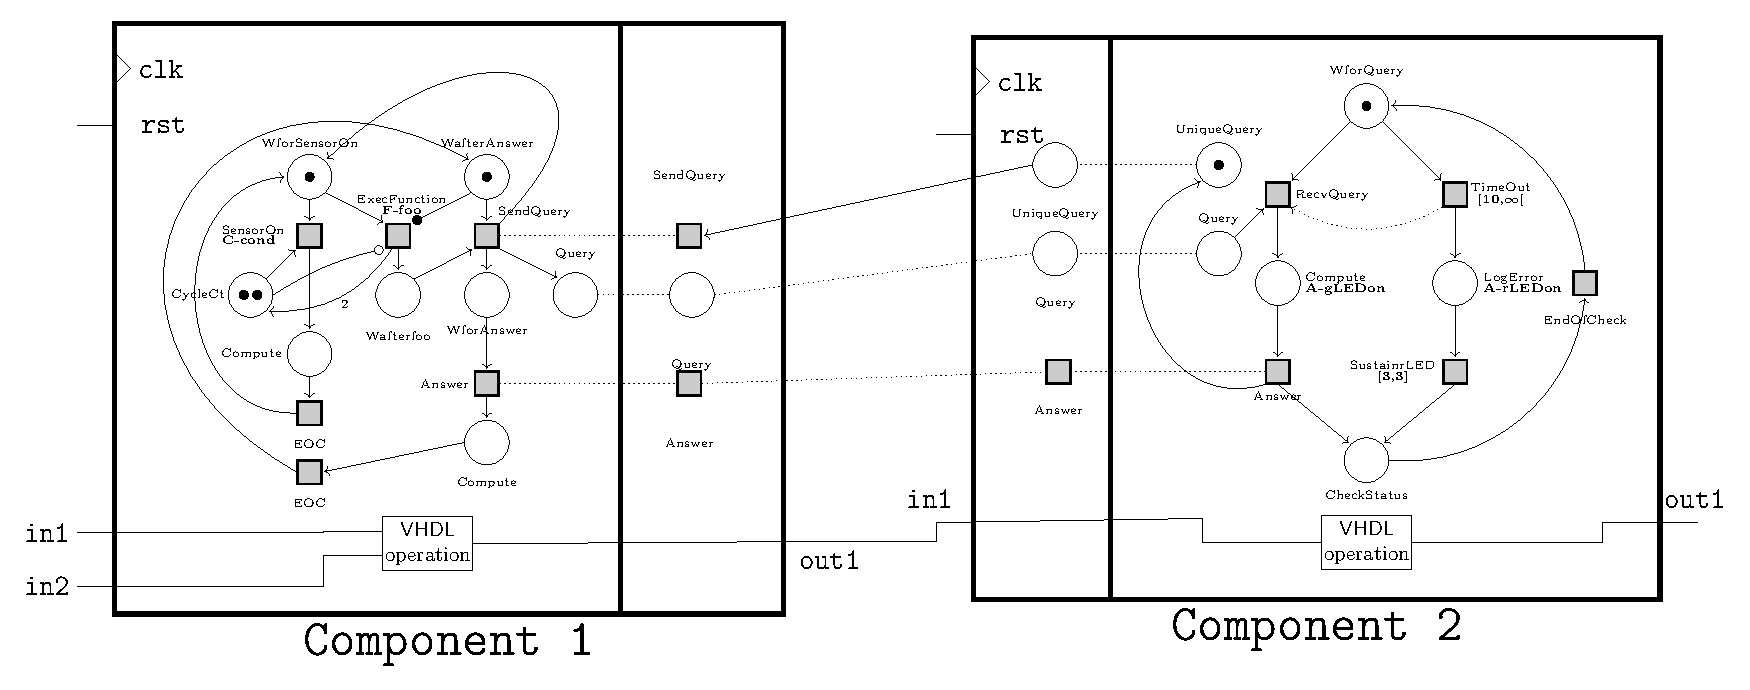
\includegraphics[keepaspectratio=true,width=\textwidth]{abs-model.eps}
\caption[An example of model of digital system in \hilecop{}.]{A
  component-based model of digital system in \hilecop{}.}
\label{fig:abs-model}
\end{figure}

In \hilecop{}'s high-level formalism, a model of digital system is
composed of boxes that represent the different components of the
system. Figure~\ref{fig:abs-model} gives an example of such a model.
The internal behavior of each component is defined by an SITPN model.
The elements of a component's internal behavior can be connected to
the elements of another component's behavior through an interface. Two
elements are either connected through a place-transition (or
transition-place) arc, or through a fusion arc (dotted line in
Figure~\ref{fig:abs-model}). While designing a component, an engineer
can also define input and output ports in the component interface,
declare internal signals, and perform operations over the ports and
internal signals by writing \vhdl{} code. All the \vhdl{} code defined
in this way will be copied as is in the output \vhdl{} design during
the model-to-text transformation. Note that all components declare a
clock and a reset signal (cf. \texttt{clk} and \texttt{rst} in
Figure~\ref{fig:abs-model}). These signals are related to the
synchronous execution of the system in the final physical device.

Before being transformed into \vhdl{} code, the model is flattened
down (cf. Step \circled{1} to step \circled{2} in
Figure~\ref{fig:hilecop-wf}). All component structures are removed,
and the result is one global SITPN model. During this flattening step,
all elements that were connected through fusion arcs are merged
together. Figure~\ref{fig:impl-model} presents the global SITPN model
resulting from the flattening of the component-based model of
Figure~\ref{fig:abs-model}.

\begin{figure}[H]
\centering
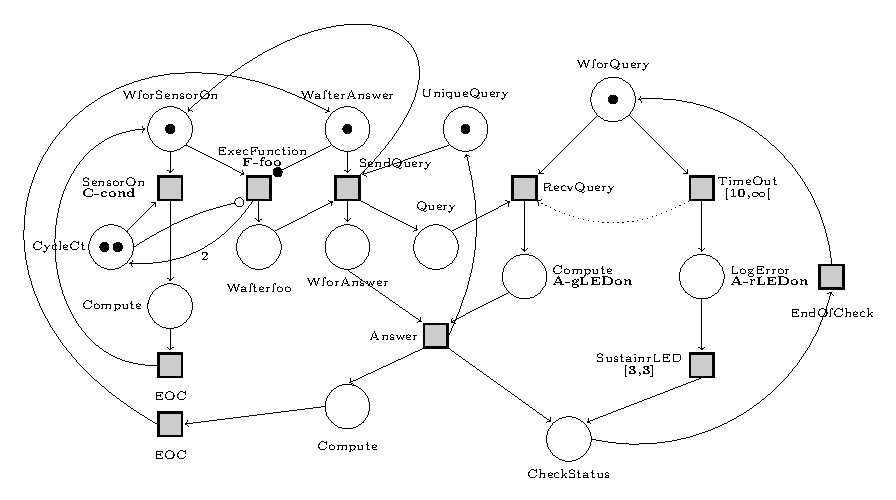
\includegraphics[keepaspectratio=true,width=\textwidth] {impl-model.eps}
\caption[Global Petri net model.]{A global Petri net model obtained
  after the flattening of a \hilecop{} high-level model.}
\label{fig:impl-model}
\end{figure}

SITPNs are a combination of multiple classes of PNs, namely: extended
PNs, generalized PNs, interpreted PNs, time PNs and PNs with
priorities. A generalized Petri net admits the weight of its arcs to
be a natural number instead of the default value of one (i.e. when no
number is written above the arc). An extended Petri net introduces two
kind of place-transition arcs, the \textit{inhibitor} arc,
characterized by a white circle head, and the \textit{test} arc, which
has a black circle head. These arcs condition the firing of a
connected transition, however, they do not cause tokens to be removed
from input places at firing time. In Figure~\ref{fig:impl-model}, the
arc from place CycleCt to transition ExecFunction is an inhibitor arc,
and the arc from place WafterAnswer to ExecFunction is a test arc.
Now, let us introduce more specifically the class of interpreted PNs,
time PNs and PNs with priorities.

\paragraph{Interpreted Petri nets}
% As stated in \cite{David1994}, Interpreted Petri Nets (IPN) ``can be
% applied to various interpretations according to the use wished to be
% made of it''.
In its general definition \cite{David1994}, an IPN is associated with
a finite set of variables $V$, a finite set of operations $O$, and a
finite set of conditions $C$. Operations of the $O$ set are associated
with places and triggered when the places become marked. The execution
of operations affects the value of the variables, and the value of
conditions depends on Boolean expressions computed upon the variables.
Conditions are associated with transitions and become involved in the
firing process.  In the \hilecop{} version of
IPNs, % refines the concepts of the general
% definition. In this version, 
the set of variables corresponds to the set of \vhdl{} signals that
are handled by the model; a signal can be an input port, an output
port or an internal signal of the modeled hardware circuit. The
operations, implemented by \vhdl{} procedures, are separated in two
kinds, namely: actions and functions. Actions (or continuous
operations) are associated to the places; all the actions associated
to a place $p$ are activated as long as $p$ is marked (i.e. as long as
$p$ holds a token). Functions (or discrete operations) are associated
to the transitions; when a transition $t$ is fired, all functions
associated to $t$ are executed once. In Figure \ref{fig:impl-model},
\textbf{C-cond} is a condition associated to the transition SensorOn;
\textbf{F-foo} is a function associated to the transition
ExecFunction; \textbf{A-gLEDon} and \textbf{A-rLEDon} are two actions
associated to the Compute and LogError places.
% Figure~\ref{fig:ipn} illustrates the use of actions, functions and
% conditions in an interpreted Petri net as applied in the \hilecop{}
% high-level models.

% \begin{figure}[H]
%   \centering
%   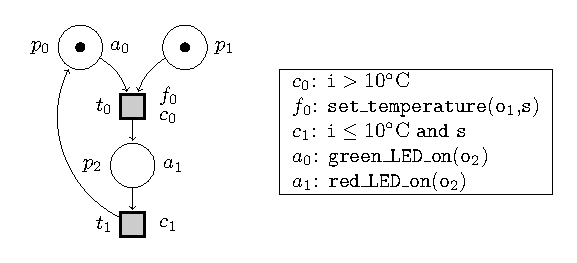
\includegraphics[keepaspectratio=true, width=.7\textwidth]{interpreted-pn.eps}
%   \caption[An example of Interpreted Petri net.]{An example of
%     interpreted Petri net; on the left side, the interpreted Petri
%     net; on the right side, examples of tests associated to conditions
%     and operations associated to actions and functions.}
%   \label{fig:ipn}
% \end{figure}%
% %
% In Figure~\ref{fig:ipn}, the set of \vhdl{} signals, on which the
% interpretation elements act upon, is
% $\{\mathit{i}, \mathtt{s}, \mathtt{o}_1, \mathtt{o}_2\}$. Here, signal
% \texttt{i} is an input port of the hardware, \texttt{s} is an internal
% signal, and \texttt{o}$_1$ and \texttt{o}$_2$ are two output
% ports. The action $a_0$ is activated as place $p_0$ is marked; thus,
% the operation \texttt{green\_LED\_on}(\texttt{o}$_2$) is currently
% executed. Also, function $f_0$ will be executed (i.e. operation
% \texttt{set\_temperature}(\texttt{o}$_1$, \texttt{s})) at the firing
% of $t_0$% , that is if condition $c_0$ is \texttt{true} and $t_0$ is
% % sensitized
% . On the right side of Figure~\ref{fig:ipn}, we associate Boolean
% expressions with conditions; these expressions depend on the value of
% the signals declared by the model. Also, we associate actions and
% functions with operations that handle the signals of the model which
% are passed as inputs. Concretely, in the \hilecop{} high-level models,
% functions and actions are declared as \vhdl{}
% procedures. Listing~\ref{lst:vhdl-fun} gives one possible
% implementation of the \texttt{set\_temperature} operation as a \vhdl{}
% procedure; the \texttt{set\_temperature} operation is associated with
% function $f_0$ in Figure~\ref{fig:ipn}.

% \begin{lstlisting}[language=vhdl,
% caption={[An example of \vhdl{} procedure implementing a function.]An example of \vhdl{} procedure implementing the operation \texttt{set\_temperature} associated with the function $f_0$.},label={lst:vhdl-fun},framexleftmargin=1.5em,xleftmargin=2em,numbers=left,numberstyle=\tiny\ttfamily]
% procedure set_temperature(signal tmp : out integer; signal flag : inout std_logic) is
% begin
%   if flag = '1' then
%     tmp <= 30;
%     flag <= '0';
%   else 
%     tmp <= 10;
%     flag <= '1';
%   endif;
% end set_temperature;
% \end{lstlisting}

% In Listing~\ref{lst:vhdl-fun}, the \texttt{set\_temperature} procedure
% declares two parameters: the \texttt{tmp} signal which is a write-only
% signal of type \texttt{integer}, and the \texttt{flag} signal which is
% a both readable and writable signal of the Boolean type
% (\texttt{std\_logic} in \vhdl{}). The \texttt{set\_temperature}
% procedure checks the value of the \texttt{flag} signal and assigns a
% new value to the \texttt{tmp} and \texttt{flag} signals
% accordingly.
% The $\Leftarrow$ operator is the assignment operator for
% signals in the \vhdl{} syntax (more on that in
% Section~\ref{sec:hvhdl}).

\paragraph{Time Petri nets}

In a time Petri net (TPN), time intervals can be associated to
transitions, along with a dynamic time counter value. Thus, the firing
of a transition must happen in a certain time window. In the
\hilecop{} version of TPNs, time intervals are of the form $[a, b]$,
where $a\in\mathbb{N}^{*}$ and
$b\in\mathbb{N}^{*}\sqcup\{\infty\}$. % Other definitions of time
% intervals exist for TPNs (e.g. with real numbers), but here we will
% only consider the latter definition.
In Figure~\ref{fig:impl-model},
transitions SustainrLED and TimeOut are both associated with time
intervals.

\paragraph{Petri nets with priorities}

Two transitions are in structural conflict if they have a common input
place connected through a \textit{basic} arc (i.e. neither inhibitor
nor test arc). When two transitions in structural conflict are firable
at the same time and if the firing of one of the transitions disables
the other, then, the conflict becomes \textit{effective}. In a Petri
net with priorities, it is possible to specify a firing priority in
the case where the conflict between two transitions becomes
effective. In that case, the transition with the highest firing
priority will always be fired first. In Figure \ref{fig:impl-model},
the fact that transition TimeOut has a higher firing priority than
transition RecvQuery is graphically represented by a dotted arrow. \\

\noindent{}Now let us formally introduce the structure of SITPNs:

\begin{definition}[SITPN]
  \label{def:sitpn}
  A synchronously executed, extended, generalized, interpreted, and
  time Petri net with priorities is a tuple
  ${<}P,T,pre,post,M_0,{\succ},\mathcal{A},\mathcal{C},\mathcal{F},
  \mathbb{A},\mathbb{C},\mathbb{F},{I_s}{>}$, where we have:
  % 
  \begin{enumerate}
  \item $P=\{p_0,\ldots,p_n\}$, a finite set of places.
  \item $T=\{t_0,\ldots,t_m\}$, a finite set of transitions.
  \item
    $pre\in{}P\rightarrow{}T\nrightarrow(\mathbb{N}^{*}\times\{\mathtt{basic},\mathtt{inhib},\mathtt{test}\})$,
    the function associating a weight and a type to place-transition
    edges.
  \item $post\in{}T\rightarrow{}P\nrightarrow\mathbb{N}^{*}$, the
    function associating a weight to transition-place edges.
  \item $M_0\in{}P\rightarrow\mathbb{N}$, the initial marking of the SITPN.
  \item $\succ\subseteq{}(T\times{}T)$, the priority relation, which
    is a strict partial order over the set of transitions.
  \item $\mathcal{A}=\{a_0,\ldots,a_i\}$, a finite set of continuous actions.
  \item $\mathcal{F}=\{f_0,\ldots,f_k\}$, a finite set of functions.
  \item $\mathcal{C}=\{c_0,\ldots,c_j\}$, a finite set of conditions.
  \item $\mathbb{A}$ $\in$ ${}P$ $\rightarrow$ $\mathcal{A}$
    $\rightarrow$ $\mathbb{B}$, the function associating actions to
    places.  $\forall{}p\in{}P$, $\forall{}a\in\mathcal{A}$,
    $\mathbb{A}(p,a)=\mathtt{true}$, if $a$ is associated to $p$,
    $\mathbb{A}(p,a)=\mathtt{false}$ otherwise.
  \item $\mathbb{F}\in{}T\rightarrow\mathcal{F}\rightarrow\mathbb{B}$,
    the function associating functions to transitions.
    $\forall{}t\in{}T,~\forall{}f\in\mathcal{F},$
    $\mathbb{F}(t,f)=\mathtt{true}$, if $f$ is associated to $t$,
    $\mathbb{F}(t,f)=\mathtt{false}$ otherwise.
    
  \item $\mathbb{C} \in T \rightarrow \mathcal{C} \rightarrow\{-1,0,1\}$, the
    function associating conditions to transitions.
    $\forall t \in T$, $\forall c \in \mathcal{C}$,
    $\mathbb{C}(t,c)=1$, if $c$ is associated to $t$,
    $\mathbb{C}(t,c)=-1$, if $\bar{c}$ is associated to $t$,
    $\mathbb{C}(t,c)=0$ otherwise.
  \item
    $I_s\in{}T\nrightarrow(\mathbb{N}^{*}\times(\mathbb{N^{*}}\sqcup\{\infty\}))$,
    the partial function associating time intervals to transitions.
  \end{enumerate}
\end{definition}

% In Definition~\ref{def:sitpn}, the structure holds the \textit{static}
% elements of a SITPN model, i.e. all the elements which value does not
% evolve with the execution of the model. Therefore, the value of time
% counters associated with transitions does not appear in the SITPN
% structure. As the value of time counters is \textit{dynamic}, i.e. it
% evolves with the execution of an SITPN model, it is a part of the
% SITPN state.

In Definition~\ref{def:sitpn}, we do not consider the set of \vhdl{}
signals manipulated by a SITPN model. As a consequence, the structure
holds neither the association between conditions and Boolean
expressions, and nor the association between actions/functions and
operations (i.e. \vhdl{} procedures that act upon signal values).  In
this simplified version of the SITPN structure, conditions, actions
and functions are only considered as finite sets of indexed elements
associated with the places and transitions of an SITPN.

Note also that the priority relation (Item~6 of
Definition~\ref{def:sitpn}) is a partial order over the set of
transitions. Establishing a firing priority is only necessary between
transitions in structural conflict.

% In a TPN, a dynamic time counter
% value is associated to transitions with a time interval

% In Figure~\ref{fig:tpn}, time
% counters are represented in red between diamond brackets. The current
% value of time counters is part of the state of the TPN, along with its
% current marking, whereas time intervals are part of the static
% structure of the TPN.

% \begin{figure}[H]
%   \centering
%   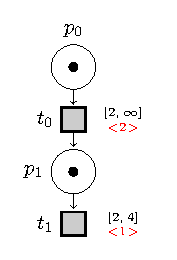
\includegraphics[keepaspectratio=true, width=0.2\textwidth]{time-pn.eps}
%   \caption[An example of time Petri net.]{An example of time Petri
%     net. The value of time counters appears between diamond brackets.}
%   \label{fig:tpn}
% \end{figure}
% For each sensitized transition associated with a time interval, time
% counters are incremented at a certain time step, previously defined by
% the designer. For instance, in the case of SITPNs, i.e. Petri nets
% used in the \hilecop{} methodology, the reference time step for the
% increment of time counters is the clock cycle.

% When a transition associated with a time interval is fired or
% disabled, a reset order is sent to the transition to set its time
% counter value to
% zero.
% In time Petri nets, a transition is firable if:
% \begin{itemize}[label=--]
% \item It is enabled.
% \item Its time counter value is within its time interval.
% \end{itemize}

% For instance, in Figure~\ref{fig:tpn}, only transition $t_0$ is
% firable.
% There are several possible firing policies for TPNs. Here, we will
% only consider the \textit{imperative} firing policy: as soon as a time
% counter reaches the lower bound of a time interval, the associated
% transition must be fired if all the other firability conditions are
% verified.

% Figure~\ref{fig:structural-conflict} illustrates the
% application of a priority relation to solve the effective conflict
% between two transitions.

% \begin{figure}[H]
%   \centering
%   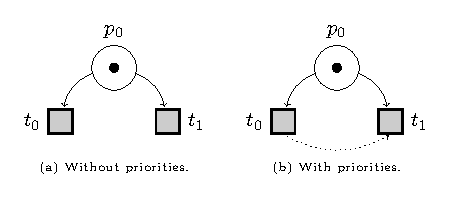
\includegraphics[keepaspectratio=true,width=.6\textwidth]{structural-conflict.eps}
%   \caption[An example of transitions in structural and effective
%   conflict.]{An example of transitions in structural and effective
%     conflict. In subfigure (b), the dotted arrow represents the
%     priority relation between $t_0$ and $t1$. The transition with the
%     highest firing priority is at the source of the arrow; here,
%     transition $t_0$.}
%   \label{fig:structural-conflict}
% \end{figure}

\subsection{Synchronous execution semantics}
\label{subsec:hpn-particularities}

% The aspect of SITPNs that constitutes the originality of the formalism
% compared to the standard PN semantics is its synchronous execution.
% The class of interpreted Petri nets increases the expressiveness of
% the \hilecop{} high-level models. However, to ensure the safe
% execution of functions after synthesis on a physical device, the whole
% system must be synchronized with a clock signal \cite{Leroux2014}. As
% a consequence, a clock signal regulates the evolution of SITPNS
% (i.e. it is a part of their semantics). 
 The SITPN semantics describes
the evolution of the state of an SITPN through a given number of clock
cycles; thus, we must first define the SITPN state structure. In what
follows, for a given $sitpn\in{}SITPN$, $T_i$ denotes the definition
domain of $I_s$, i.e. the set of transitions associated with a time
interval, referred to as \textit{time transitions}.

\begin{definition}[SITPN State]
  \label{def:sitpnstate}
  For a given $sitpn\in{}SITPN$, let $S(sitpn)$ be the set of possible
  states of $sitpn$. An SITPN state $s\in{}S(sitpn)$ is a tuple
  ${<}M,I,reset_t,ex,cond{>}$, where:
  \begin{enumerate}
  \item $M\in{}P\rightarrow\mathbb{N}$ is the current marking of
    $sitpn$.
  \item\label{item:sitpn-state-tc} $I\in{}T_i{}\rightarrow\mathbb{N}$
    is the function mapping time transitions to their current time
    counter value.
  \item\label{item:sitpn-state-rst}
    $reset_t\in{}T_i\rightarrow\mathbb{B}$ is the function mapping
    time transitions to time counter reset orders (defined as
    Booleans).
  \item $ex\in{}\mathcal{A}\sqcup\mathcal{F}\rightarrow\mathbb{B}$ is
    the function representing the current activation (resp. execution)
    state of actions (resp. functions).
  \item $cond\in\mathcal{C}\rightarrow\mathbb{B}$ is the function representing the
    current value of conditions (defined as Booleans).
  \end{enumerate}
\end{definition}

As described in Definition~\ref{def:sitpnstate}, the state of a SITPN
is characterized by its marking, the value of time counters, the reset
orders assigned to time counters, the execution/activation status of
actions/functions (Boolean values), and the value of conditions (also
Boolean). Regarding actions and functions, note that we are only
interested in the fact that a given action/function is
activated/executed but no more in actually executing the associated
operation.

Before defining the SITPN state transition relation, let us formally
introduce the definition of the sensitization of a given transition by
a given marking, and the definition of the firability of a given
transition with respect to a given SITPN state.

\begin{definition}[Sensitization]
  \label{def:sens}
  A transition $t\in{}T$ is said to be sensitized, or enabled, by a
  marking $M$, which is noted $t\in{}Sens(M)$, if
  $\forall{}p\in{}P,\forall\omega\in\mathbb{N}^{*},~\big(pre(p,t)=(\omega,\mathtt{basic})\vee{}pre(p,t)=(\omega,\mathtt{test})\big)\Rightarrow{}M(p)\ge{}\omega$,
  and $pre(p,t)=(\omega,\mathtt{inhib})\Rightarrow{}M(p)<{}\omega$.
\end{definition}

\begin{definition}[Firability]
  \label{def:firable}
  A transition $t\in{}T$ is said to be firable at a state
  $s={<}M,I,reset_t,ex,cond{>}$, which is noted $t\in{}Firable(s)$, if
  $t\in{}Sens(M)$, and $t\notin{}T_i$ or $I(t)\in{}I_s(t)$, and
  $\forall c \in \mathcal{C}, \mathbb{C}(t, c) = 1 \Rightarrow cond(c)
  = 1$ and $\mathbb{C}(t, c) = -1 \Rightarrow cond(c) = 0$.
\end{definition}

When a transition $t$ is firable at a given SITPN state $s$, and if
$t$ is a top-priority transition (i.e. there exists no transition with
a higher firing priority than $t$), then $t$ belongs to the set of
\textit{fired} transitions at state $s$.  When a transition $t$ is
involved in a structural conflict solved with priorities, $t$ is
firable at a given state $s$ is no longer equivalent to $t$ is fired
at $s$.  As illustrated in Figure~\ref{fig:resid-marking}, to
determine which transitions of $t_0$, $t_1$ and $t_2$ must be fired, a
\emph{residual marking} is computed by following the priority
order. For each transition of the group $t_0$, $t_1$ and $t_2$, the
residual marking represents the remaining tokens in $p_0$ after the
firing of transitions with a higher firing priority. To be fired, a
transition must be firable \emph{and} must be enabled by the residual
marking. Thus, the recursive definition of the set of fired
transitions at a given SITPN state is as follows:

\begin{definition}[Fired]
  \label{def:fired}
  A transition $t\in{}T$ is said to be fired at the SITPN state
  $s={<}M,I,reset_t,ex,$ $cond{>}$, which is noted $t\in{}Fired(s)$,
  if $t\in{}Firable(s)$ and
  $t\in{}Sens\big(M-\sum\limits_{t_i\in{}Pr(t)}pre(t_i)\big)$, where
  $Pr(t)=\{t_i~|~t_i\succ{}t\wedge{}t_i\in{}Fired(s)\}$.
\end{definition}

The computation of the residual marking only involves the consumption
phase of the firing process; tokens are withdrawn from places, but
none are generated.

\begin{figure}[H]
  \centering
  \includegraphics[keepaspectratio=true, width=.9\textwidth]{resid-marking.eps}
  \caption[Computation of the residual marking of a group of
  conflicting transitions.]{Computation of the residual marking for a
    group of conflicting transitions. At \circled{1}
    (resp. \circled{2} and \circled{3}), place $p_0$ holds the
    residual marking for transition $t_0$ (resp. $t_1$ and
    $t_2$). Condition $c_0$ appears in normal font to indicate that
    its current value is \texttt{false}.}
  \label{fig:resid-marking}
\end{figure}

% Figure~\ref{fig:sync-exec} depicts the process of state evolution,
% following the clock signal.

% \begin{figure}[H]
%   \centering
%   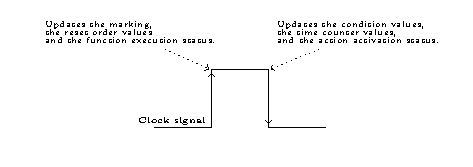
\includegraphics[keepaspectratio=true, width=.9\textwidth]{sync-exec.eps}
%   \caption{Evolution of an SITPN synchronized with a clock signal.}
%   \label{fig:sync-exec}
% \end{figure}

\paragraph{The state transition relation}

The evolution of the state of a SITPN is \textit{synchronized} with
the rising edge event and the falling edge event of a clock signal.
% As shown in Figure~\ref{fig:sync-exec}, the state evolution process
% of a SITPN is divided into two steps.
The rising edge event triggers the marking update, which is the
consequence of transition firing; all time transitions that have been
fired or disabled by the firing process receive time counter reset
orders; all functions associated with fired transitions are
executed. On the falling edge of the clock signal, the value of
conditions are updated. As the SITPN structure does not hold the link
between Boolean expressions computed over \vhdl{} signals and
conditions, the update of condition values is represented by the
injection of fresh Boolean values coming from an
environment. Moreover, the falling edge event triggers the evolution
of the time counter values; values are incremented, reset, or stalling
in the case where a time counter has reached the upper bound of its
associated time interval. Finally, all actions associated with marked
places are activated. Figure~\ref{fig:sitpn-state-exec} gives an
example of the evolution of the state of a given SITPN through one
clock cycle, happening in the middle of other clock cycles. % The
% aim of this figure and the explanation that follows is to give some
% hints to the reader about the semantics of SITPNs before giving its
% formal definition in Section~\ref{sec:sitpn-sem}.

\begin{figure}[H]
  \centering
  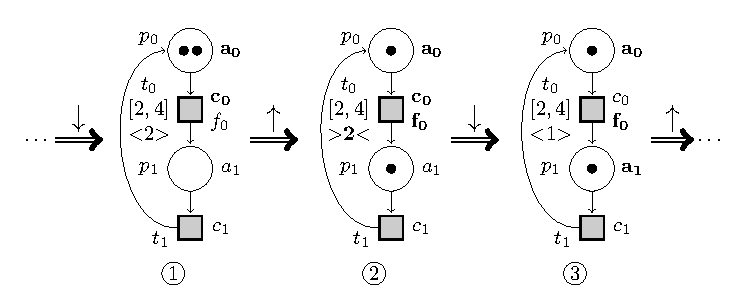
\includegraphics[keepaspectratio=true, width=.9\textwidth]{sitpn-state-evol.eps}
  \caption[Evolution of an SITPN over one clock cycle.]{The evolution
    of a SITPN over one clock cycle. Conditions (i.e. $c_0$ and $c_1$)
    appear in bold font when \texttt{true}; actions (i.e. $a_0$ and
    $a_1$) and functions ($f_0$) appear in bold font when
    activated/executed; time counters appear between diamond brackets,
    and are represented between inverted brackets when they are
    subject to a reset order.}
  \label{fig:sitpn-state-exec}
\end{figure}

In Figure~\ref{fig:sitpn-state-exec}, from Step~1 to Step~2, the
rising edge of the clock signal triggers the firing of transition
$t_0$. % At Step~1, transition $t_0$ gathers all the necessary
% conditions to trigger the firing process. Transition $t_0$ is said to
% be \textit{firable}, namely:

% \begin{itemize}[label=--]
% \item $t_0$ is sensitized, or enabled, by the current marking.
% \item Condition $c_0$ is \texttt{true} (appears in bold font).
% \item The value of $t_0$'s time counter is within the associated time
%   interval ($2\in[2,4]$).
% \end{itemize}


% In Figure~\ref{fig:sitpn-state-exec},
As transition $t_0$ is firable and is not in effective conflict with
other transitions, $t_0$ is fired: one token is consumed in place
$p_0$ and one token is produced in place $p_1$. Also, function $f_0$
is executed at the occurrence of the rising edge of the clock signal,
and thus, $f_0$ appears in bold font at Step~2. Consequently to the
firing of $t_0$, a reset order is sent to the time counter of $t_0$,
and it appears between inverted brackets at Step~2. From Step~2 to
Step~3, the falling edge updates the action activation status: $a_0$
stays activated as place $p_0$ is still marked; $a_1$ becomes newly
activated as place $p_1$ just received a token. Time counters are
updated: $t_0$'s time counter is set to zero as the transition
previously received a reset order. However, as $t_0$ is still enabled
by the new marking, its time counter is incremented. Thus, the
resulting time counter value at Step~3 is of one (i.e. result of reset
plus increment). Also, the environment provides a new value to each
condition. As a consequence, condition $c_0$ takes the value
\texttt{false} and condition $c_1$ keeps the same value.

We formalize the evolution of a SITPN state synchronized with the
events of a clock signal with the following state transition relation:

\begin{definition}[SITPN state transition relation]
  \label{def:semantics}
  % \begin{itemize}[label=-]
  % \item
  %   $E_c\in{}\mathbb{N}\rightarrow\mathcal{C}\rightarrow\mathbb{B}$ is
  %   the environment function, which gives (Boolean) values to
  %   conditions ($\mathcal{C}$) depending on the count of clock cycles
  %   ($\mathbb{N}$).
  % \item $\rightarrow\subseteq{}S(sitpn)\times{}L\times{}S(sitpn)$ is the SITPN state
  %   transition relation
  The SITPN state transition relation
  $\rightarrow\subseteq{}(\mathbb{N}\rightarrow\mathcal{C}\rightarrow\mathbb{B})\times{}S(sitpn)\times{}\mathbb{N}\times{}\{\uparrow,\downarrow\}\times{}S(sitpn)$, which is noted\\
  $E_c,\tau\vdash{}s\xrightarrow{clk}s'$ where
  $E_c\in\mathbb{N}\rightarrow\mathcal{C}\rightarrow\mathbb{B}$,
  $\tau\in\mathbb{N}$, $s,s'\in{}S(sitpn)$ and
  $clk\in\{\uparrow,\downarrow\}$, is defined as follows:
  
  \begin{itemize}
  \item
    $\forall{}E_c\in\mathbb{N}\rightarrow\mathcal{C}\rightarrow\mathbb{B}$,
    $\forall\tau\in\mathbb{N}$, $\forall{}s,s'\in{}S(sitpn)$, we have
    $E_c,\tau\vdash{}s\xrightarrow{\downarrow}s'$, where
    $s=<M,I,reset_t,ex,cond>$ and $s'=<M,I',reset_t,ex',cond'>$, if:
    \begin{enumerate}[]
    \item\label{it:cond-env} $cond'$ is the function giving the
      (Boolean) values of conditions that are extracted from the
      environment $E_c$ at the clock count
      $\tau$, i.e.:
      \begin{equation*}
        \forall{}c\in{}\mathcal{C},~cond'(c)=E_c(\tau,c).
      \end{equation*}
      
    \item\label{it:activate-actions} All the actions associated
      with at least one
      marked place in the marking $M$ are activated, i.e.:
      \begin{equation*}
        \forall{}a\in{}\mathcal{A},~ex'(a)=\sum\limits_{p\in{}marked(M)}\mathbb{A}(p,a)
        ~where~marked(M)=\{p'\in{}P~\vert~M(p')>0\}.
      \end{equation*}
    \item\label{it:reset-counters} All the time transitions that are
      sensitized by the marking $M$ and received the order to reset
      their time intervals, have their time counter reset and
      incremented, i.e.:
      \begin{equation*}
        \forall{}t\in{}T_i,~t\in{}Sens(M)\land{}reset_t(t)=\mathtt{true}
        \Rightarrow{}I'(t)=1.
      \end{equation*}
      
    \item\label{it:inc-counters} All the time transitions that are
      sensitized by the marking $M$, and
      did not receive a reset order, increment their time counters if time counters are still active, i.e.:
      \begin{equation*}
        \begin{split}
          \forall{}t\in{}T_i,~&t\in{}Sens(M)\land{}reset_t(t)=\mathtt{false}\land{}[I(t)\le{}u(I_s(t))\lor{}u(I_s(t))=\infty]\\
                              & \Rightarrow{}I'(t)=I(t)+1. \\
        \end{split}
      \end{equation*}
    \item\label{it:locked-counters} All the time transitions
      verifying the same
      conditions as above, but with locked counters, keep having locked counters (values are stalling), i.e.:        
      \begin{equation*}
        \begin{split}
          \forall{}t\in{}T_i,~&t\in{}Sens(M)\land{}reset_t(t)=\mathtt{false}\land{}I(t)>{}u(I_s(t))\land{}u(I_s(t))\neq\infty\\
                              & \Rightarrow{}I'(t)=I(t).\\
        \end{split}
      \end{equation*}
      
    \item\label{it:reset-not-sens} All the time transitions disabled by the marking $M$ have their time counters set to zero, i.e.:
      \begin{equation*}
        \forall{}t\in{}T_i,~t\notin{}Sens(M)\Rightarrow{}I'(t)=0.
      \end{equation*}
    \end{enumerate}
    
  \item $\forall\tau\in\mathbb{N}$, $\forall{}s,s'\in{}S(sitpn)$, we
    have $E_c,\tau\vdash{}s\xrightarrow{\uparrow}s'$, where
    $s=<M,I,reset_t,ex,cond>$ and $s'=<M',I,reset_t',ex',cond>$, if:
    \begin{enumerate}[% label=(\arabic*),
      resume]
    \item\label{it:new-marking} $M'$ is the new marking resulting
      from
      the firing of all the transitions contained in $Fired(s)$, i.e.:
      \begin{equation*}
        \forall{}p\in{}P,~M'(p)=M(p)-\sum\limits_{t\in{}Fired(s)}pre(p,t)+\sum\limits_{t\in{}Fired(s)}post(t,p).
      \end{equation*}
      
    \item\label{it:reset-order} A time transition receives a reset
      order if it is fired at state $s$, or, if there exists a place
      $p$ connected to $t$ by a \texttt{basic} or \texttt{test arc}
      and at least one output transition of $p$ is fired and the
      transient marking of $p$ disables $t$; no reset order is sent
      otherwise:
      \begin{equation*}
        \begin{split}
          \forall{}t\in{}T_i,&~t\in{}Fired(s) \\
                             &\lor\big(\exists{}p\in{}P,\omega\in\mathbb{N}^{*}, \\
                             &\quad\quad{}[pre(p,t)=(\omega,\mathtt{basic})\lor{}pre(p,t)=(\omega,\mathtt{test})] \\
                             &\quad\quad\land\sum\limits_{t_i\in{}Fired(s)}pre(p,t_i)>0 \\
                             &\quad\quad\land{}M(p)-\sum\limits_{t_i\in{}Fired(s)}pre(p,t_i)<\omega\big)\\
                             & \Rightarrow{}reset'_t(t)=\mathtt{true}~and~reset'_t(t)=\mathtt{false}~otherwise.  \\
        \end{split}
      \end{equation*}
      
    \item\label{it:exec-fun} All functions associated with at least one fired transition are executed, i.e:
      \begin{equation*}
        \forall{}f\in{}\mathcal{F},~ex'(f)=\sum\limits_{t\in{}Fired(s)}\mathbb{F}(t,f).
      \end{equation*}
    \end{enumerate}
  \end{itemize}
\end{definition}


% In Figure~\ref{fig:resid-marking}, the residual marking for $t_0$
% corresponds to the marking obtained after the firing of all
% transitions with a higher priority. As $t_0$ is the transition with
% the highest firing priority, the residual marking for $t_0$ is equal
% to the current marking. Transition $t_0$ gathers all the conditions to
% be firable and is enabled by the residual marking; thus, $t_0$ will be
% fired on the next rising edge. The residual marking for $t_1$ is the
% marking obtained after the firing of $t_0$, i.e. the only transition
% with a higher priority. As illustrated at \circled{2}, $t_1$ is
% enabled by the residual marking. However, $t_1$ does not gather all
% the conditions to be firable as the value of condition $c_0$ is
% \texttt{false}. Thus, $t_1$ will not be fired on the next rising
% edge. The residual marking for $t_2$ is obtained after the firing of
% $t_0$ only. Even though transition $t_1$ has a higher firing priority
% than $t_2$, $t_1$ is not a member of the set of fired transitions.
% Thus, $t_1$ is not taken into account in the computation of the
% residual marking for $t_2$. The residual marking at \circled{3}
% enables transition $t_2$, and as $t_2$ gathers all the conditions to
% be firable, then $t_2$ will be fired on the next rising edge.

% \paragraph{Locked time counters}

% SITPNs inherit the properties of time PNs and interpreted PNs. The
% phenomenon of \emph{locked} time counters is a consequence of this
% inheritance. As illustrated in Figure~\ref{fig:locked-tc}, the value
% of a time counter can overreach the upper bound of its associated time
% interval. This situation can only arise if a condition hinders the
% firing of a given transition while the considered transition is still
% enabled by the marking. As a consequence, the time counter will be
% incremented at every clock cycle until the upper bound of the time
% interval is overreached. Then, at this point, the time counter is said
% to be \emph{locked} and its value will no more evolve.

% \begin{figure}[H]
%   \centering
%   \includegraphics[keepaspectratio=true, width=.45\textwidth]{locked-tc.eps}
%   \caption[An example of locked time counter.]{An example of locked
%     time counter. Condition $c$ is equal to \texttt{false} and thus
%     appears in \textcolor{red}{red}.}
%   \label{fig:locked-tc}
% \end{figure}

% In Figure~\ref{fig:locked-tc}, condition $c$ is valuated to
% \texttt{false} before the falling edge of the clock signal. Thus,
% transition $t$ can not be fired but is still enabled by the
% marking. On the next falling edge, the time counter of transition $t$
% is incremented and overreaches the upper bound of interval $[2,4]$ and
% thus becomes locked. If the designer of the model has not anticipated
% the case of a locked time counter, and has not provided an alternative
% to disable place $p$ in that case, then the transition $t$ will never
% be firable again.

\todo[inline]{Put what follows in section well-definition of a SITPN
  model.}

The synchronous execution semanctics of SITPNs implies that all
transitions are fired at the same time. In
Figure~\ref{fig:double-consum}, transitions $t_0$ and $t_1$ are both
firable before the rising edge event, and consequently are both fired
at the occurrence of the event. The system acts as if two tokens were
available in place $p_0$, one for the firing of $t_0$ and another for
the firing of $t_1$.

\begin{figure}[H]
  \centering
  \includegraphics[keepaspectratio=true, width=.6\textwidth]{double-consum.eps}
  \caption[Double consumption of token in a SITPN.]{Double consumption
    of one token in a SITPN. On the left side, the current marking
    before the firing of $t_0$ and $t_1$; on the right side, the
    marking resulting of the firing of $t_0$ and $t_1$. The arrow
    indicates the occurrence of a rising edge that triggers the firing
    process.}
  \label{fig:double-consum}
\end{figure}

In the context of a SITPN, a branching like the one of
Figure~\ref{fig:sitpn-state-exec}, normally interpreted as a
disjunctive branching, takes the semantics of a conjunctive branching
if no priority are specified between the conflicting transitions. To
avoid the phenomenon of ``double consumption'' of tokens, we enforce
the resolution of any structural conflict by means of mutual exclusion
or through the application of priorities. This policy about the
resolution of structural conflicts is part of the definition of a
\emph{well-defined} SITPN (cf. Section~\ref{sec:sitpn-wd}). The
property of well-definition is mandatory to produce safe models of
digital systems.


%%% Local Variables:
%%% mode: latex
%%% TeX-master: "main"
%%% End:

\section{A target language: \hvhdl{}}
\label{sec:hvhdl}


%%% Local Variables:
%%% mode: latex
%%% TeX-master: "main"
%%% End:

\section{Model-to-text transformation}
\label{sec:m2t}

In the following section, we present the \hilecop{} model-to-text
transformation (HM2T) through its formal specification.  The HM2T
generates a \hvhdl{} design out of an SITPN model. It also generates a
structure that relates the elements of the SITPN model to the elements
of the \hvhdl{} design. This structure is called a SITPN-to-\hvhdl{}
binder.  Its formal definition is as follows:

\begin{definition}[SITPN-to-\hvhdl{} design binder]
  \label{def:sitpn-to-hvhdl-binder}
  Given a $sitpn\in{}SITPN$ and a \hvhdl{} design $d\in{}design$, a
  SITPN-to-\hvhdl{} binder $\gamma\in{}WM(sitpn,d)$ is a tuple\\
  ${<}PMap,TMap,CMap,AFMap{>}$ where:
  \begin{itemize}
  \item $PMap\in{}P\rightarrow{}\{id_p~|~\mathtt{comp}(id_p,\mathtt{place},g,i,o)\in{}d.beh\}$
  \item $TMap\in{}T\rightarrow{}\{id_t~|~\mathtt{comp}(id_t,\mathtt{transition},g,i,o)\in{}d.beh\}$
  \item $CMap\in\mathcal{C}\rightarrow\{id_c~|~(\mathtt{in}, id_c, \mathtt{bool})\in{}d.ports\}$
  \item $AFMap\in\mathcal{A}\cup\mathcal{F}\rightarrow\{id_{af}~|~(\mathtt{out}, id_{af}, \mathtt{bool})\in{}d.ports\}$
  \end{itemize}
\end{definition}

For a given binder $\gamma$ and an element of an SITPN structure
$e\in{}P\cup{}T\cup\mathcal{C}\cup\mathcal{A}\cup\mathcal{F}$, we
write $\gamma(e)$ where $e$ is looked up in the appropriate
function. For instance, for a given $f\in\mathcal{F}$, $\gamma(f)$ is
a shorthand notation for $AFMap(f)$ where $\gamma={<}\dots,AFMap{>}$.

\bigskip

The formal specification of the HM2T is expressed as a relation
between the inputs of the transformation, namely a SITPN model and a
bounding function, and its outputs, namely a \hvhdl{} design and a
SITPN-to-\hvhdl{} binder. The relation is written
$HM2T\subseteq{}SITPN\times(P\rightarrow\mathbb{N})\times{}design\times{}WM(sitpn,d)$.
The bounding function, that is, the second parameter of the
specification relation, associates each place of the SITPN model to a
bound in terms of number of tokens. We assume that these bounds have
been obtained through the formal analysis of the input SITPN model.
The bounds represent the maximum number of tokens that a place will
possibly hold at any point of the execution of the model. Of course,
the existence of such a function implies that all the SITPN models
that are passed as inputs to the HM2T are \textit{bounded}
models\footnote{There exists no place that can accumulate an unlimited
  number of tokens in the course of the execution of the model.}. As a
matter of fact, we can prove that the HM2T is not semantic-preserving
when an unbounded SITPN model is passed as an input. The execution of
such a model will lead to an infinite incrementation of the number of
tokens in a given place. This infinite incrementation, while valid in
the mathematical world, can never be mirrored by a \vhdl{}
implementation of the model where all values must be finite.

Definition of the HM2T relation. Here only selected points of the
definition are presented and ilustrated. The full definition of the
HM2T formal specification can be found at \todo{Add ref. to formal
  spec. ref. (Arxiv or equivalent).}. We have implemented the HM2T
relation in \coq{}, and also have written a \coq{} function that
implements the transformation but is yet to be proved sound and
complete regarding its specification. % However, the
% proof of semantic preservation implies that some properties must be
% drawn regarding the implementation of the HM2T as a program.
However, all the properties that must be proved to state that the HM2T
is semantic preserving contribute to the proof of soundness of our
program w.r.t. its specification.

While expressing the HM2T relation, we refer to sets and functions
that are defined below:

\begin{itemize}
\item
  \texttt{input}$(p)=\{t~\vert~\exists\omega~s.t.~post(t,p)=\omega\}$,
  the set of input transitions of a place $p$.
\item
  \texttt{output}$(p)=\{t~\vert~\exists{}\omega,a~s.t.~pre(p,t)=(\omega,a)\}$,
  the set of output transitions of a place $p$.

\item \texttt{acts}$(p)=\{a~\vert~\mathbb{A}(p,a)=\mathtt{true}\}$,
  the set of actions associated with a place $p$.
\item
  \texttt{input}$(t)=\{p~\vert~\exists\omega,a~s.t.~pre(p,t)=(\omega,a)\}$,
  the set of input places of a transition $t$.
\item
  \texttt{output}$(t)=\{p~\vert~\exists\omega~s.t.~post(t,p)=\omega\}$,
  the set of output places of a transition $t$.
\item
  \texttt{conds}$(t)=\{c~\vert~\mathbb{C}(t,c)=1\lor\mathbb{C}(t,c)=-1\}$,
  the set of conditions associated with a transition $t$.
\item
  \texttt{trs}$(c)=\{t~\vert~\mathbb{C}(t,c)=1\lor\mathbb{C}(t,c)=-1\}$,
  the set of transitions to which a condition $c$ is associated.
\item \texttt{pls}$(a)=\{p~\vert~\mathbb{A}(p,a)=\mathtt{true}\}$, the
  set of places to which an action $a$ is associated.
\item \texttt{trs}$(f)=\{t~\vert~\mathbb{F}(t,f)=\mathtt{true}\}$, the
  set of transitions to which a function $f$ is associated.
\end{itemize}

\begin{itemize}
\item \texttt{output}$_c\in{}P\rightarrow{}2^T$.  The
  \texttt{output}$_c$ function takes a place $p$ as input and yields
  an ordered set of transitions computed as follows:
  \begin{enumerate}
  \item If all conflicts between the output transitions of $p$ are
    solved by mutual exclusion, or if the set of conflicting
    transitions of $p$ is a singleton, then \texttt{output}$_c$
    returns an empty set.
  \item Otherwise, the function tries to establish a total ordering
    over the set of conflicting transitions of $p$ w.r.t the firing
    priority relation:
    \begin{itemize}
    \item If no such ordering can be established (in that case, the
      firing priority relation is ill-formed, and the input SITPN is
      not well-defined), \texttt{output}$_c$ raises an error.
    \item Otherwise, the function returns the ordered set, with the
      top-level priority transition at the head.
    \end{itemize}
  \end{enumerate}

\item \texttt{output}$_{nc}\in{}P\rightarrow{}2^T$.  The
  \texttt{output}$_{nc}$ function takes a place $p$ as input and
  yields an unordered set of transitions computed as follows:
  \begin{itemize}
  \item If all conflicts between the output transitions of $p$ are
    solved by mutual exclusion, or if the set of conflicting
    transitions of $p$ is a singleton, then, the function returns the
    set of output transitions of $p$, i.e. \texttt{output}$(p)$ as
    defined above.
  
  \item Otherwise, the function returns the set of output transitions
    of $p$ connected through a \texttt{test} or an \texttt{inhib} arc,
    i.e.
    $\{t~\vert~\exists\omega~s.t.~pre(p,t)=(\omega,\mathtt{test})\lor{}pre(p,t)=(\omega,\mathtt{inhib})\}$.
  \end{itemize}
\end{itemize}


%%%%% Definition for the HM2T formal specification. %%%%%

\def\pdiInBeh{\mathtt{comp}(\gamma(p),\mathtt{place},g_p,i_p,o_p)\in{}d.beh}
\def\tdiInBeh{\mathtt{comp}(\gamma(t),\mathtt{transition},g_t,i_t,o_t)\in{}d.beh}

\begin{definition}[\hilecop{} model-to-text transformation specification]
  \label{def:hm2t-spec}
  For all SITPN model $sitpn\in{}SITPN$, bounding function
  $b\in{}P\rightarrow\mathbb{N}$, \hvhdl{} design $d\in{}design$, and
  SITPN-to-\hvhdl{} binder $\gamma\in{}WM(sitpn,d)$, we have
  $HM2T(sitpn,b,d,\gamma)$ if:
  
  \begin{enumerate}
  \item Design $d$ has an empty generic clause: $d.gens=\emptyset$.
    
  \item Design $d$ is elaborable in the context of the \hilecop{} design store and given an empty dimensioning function:\\
    $\exists{}\Delta\in{}ElDesign,\sigma_e\in\Sigma$ s.t.
    $\mathcal{D_\mathcal{H}},\emptyset\vdash{}d\xrightarrow{elab}\Delta,\sigma_e$.
    
  \item All the fields of the SITPN-to-\hvhdl{} binder are bijective
    functions: $PMap(\gamma)$ is bijective, $TMap(\gamma)$ is
    bijective,\dots
    
  \item For all place of the input SITPN model, there exists a
    corresponding place design instance (PDI) in the behavior of the
    \hvhdl{} design such that the identifier of the PDI is the one
    yielded
    by the binder $\gamma$:\\
    $\forall{}p\in{}P,\exists{}g_p,i_p,o_p$ s.t.  $\pdiInBeh$.
    
  \item For all place of the input SITPN model and its corresponding PDI, the generic map of the PDI holds the following associations:\\
    $\forall{}p\in{}P,g_p,i_p,o_p,\pdiInBeh\Rightarrow$\\
    $g_p=\{(\mathtt{mm}\Rightarrow{}b(p)), (\mathtt{ian}\Rightarrow
    \begin{cases}
      1~\mathrm{if}~\mathtt{input}(p)=\emptyset \\
      \vert{}\mathtt{input}(p)\vert~\mathrm{otherwise} \\
    \end{cases}),
    (\mathtt{oan}\Rightarrow
    \begin{cases}
      1~\mathrm{if}~\mathtt{output}(p)=\emptyset \\
      \vert{}\mathtt{output}(p)\vert~\mathrm{otherwise} \\
    \end{cases})\}$.
    
  \item For all place of the input SITPN model and its corresponding PDI, there is an association between the \texttt{im} input port and the initial marking of the place in the input port map of the PDI:\\
    $\forall{}p\in{}P,g_p,i_p,o_p,\pdiInBeh{}$
    $\Rightarrow(\mathtt{im}\Rightarrow{}M_0(p))\in{}i_p$.
    
  \item For all place of the SITPN model with no input transition, the
    input port map of the corresponding PDI includes the following associations:
    \begin{equation*}
      \begin{aligned}
        \forall{}p&\in{}P,g_p,i_p,o_p, \\
                  & \pdiInBeh\Rightarrow \\
                  & \mathtt{input}(p)=\emptyset\Rightarrow \\
                  & \{(\mathtt{iaw}(0)\Rightarrow{}0), (\mathtt{itf}(0)\Rightarrow{}\mathtt{false})\}\subseteq{}i_p.\\
      \end{aligned}
    \end{equation*}

  \item For all place of the SITPN model with no output transition,
    the input port map and output port map of the corresponding PDI
    includes the following associations:
    \begin{equation*}
      \begin{aligned}
        \forall{}p&\in{}P,g_p,i_p,o_p, \\
                  & \pdiInBeh\Rightarrow \\
                  & \mathtt{output}(p)=\emptyset\Rightarrow \\
                  & \{(\mathtt{oaw}(0)\Rightarrow{}0), (\mathtt{oat}(0)\Rightarrow{}\mathtt{basic}),
                    (\mathtt{otf}(0)\Rightarrow{}\mathtt{false})\}\subseteq{}i_p\\
                  & \land\{(\mathtt{oav}\Rightarrow{}\mathtt{open}), (\mathtt{pauths}\Rightarrow{}\mathtt{open}),
                    (\mathtt{rtt}\Rightarrow{}\mathtt{open})\}\subseteq{}o_p \\
      \end{aligned}
    \end{equation*}

    
  \item For all place of the SITPN model with no action, the
    \texttt{marked} output port is left unconnected in the output port
    map of the corresponding PDI:
    \begin{equation*}
      \begin{aligned}
        \forall{}p&\in{}P,g_p,i_p,o_p, \\
                  & \pdiInBeh\Rightarrow \\
                  & \mathtt{acts}(p)=\emptyset\Rightarrow \\
                  & (\mathtt{marked}\Rightarrow{}\mathtt{open})\in{}o_p \\
      \end{aligned}
    \end{equation*}

  \item For all transition of the input SITPN model, there exists a
    corresponding transition design instance (TDI) in the behavior of
    the \hvhdl{} design such that the identifier of the TDI is the one
    yielded
    by the binder $\gamma$:\\
    $\forall{}t\in{}T,\exists{}g_t,i_t,o_t$ s.t. $\tdiInBeh$.
    
  \item For all transition of the input SITPN model and its corresponding TDI, the generic map of the TDI holds the following associations:\\
    \begin{equation*}
      \begin{aligned}[t]
        \forall{}t&\in{}T,g_t,i_t,o_t, \\
                  & \tdiInBeh\Rightarrow \\
                  & g_t=\{(\mathtt{tt}\Rightarrow{}
                    \begin{cases}
                      \mathtt{NOT\_TEMPORAL}~\mathrm{if}~t\notin{}\mathtt{dom}(I_s) \\
                      \mathtt{TEMPORAL\_A\_A}~\mathrm{if}~I_s(t)=[a,a] \\
                      \mathtt{TEMPORAL\_A\_B}~\mathrm{if}~I_s(t)=[a,b] \\
                      \mathtt{TEMPORAL\_A\_INF}~\mathrm{if}~I_s(t)=[a,\infty] \\
                    \end{cases}),
        (\mathtt{mtc}\Rightarrow
        \begin{cases}
          1~\mathrm{if}~t\notin{}\mathtt{dom}(I_s) \\
          b~\mathrm{if}~I_s(t)=[a,b] \\
          a~\mathrm{if}~I_s(t)=[a,\infty] \\
        \end{cases}), \\
                  & (\mathtt{ian}\Rightarrow
                    \begin{cases}
                      1~\mathrm{if}~\mathtt{input}(t)=\emptyset \\
                      \vert{}\mathtt{input}(t)\vert~\mathrm{otherwise} \\
                    \end{cases}), 
        (\mathtt{cn}\Rightarrow
        \begin{cases}
          1~\mathrm{if}~\mathtt{conds}(t)=\emptyset \\
          \vert{}\mathtt{conds}(t)\vert~\mathrm{otherwise} \\
        \end{cases})\}. \\
      \end{aligned}
    \end{equation*}
    
  \item For all transition of the input SITPN model and its corresponding TDI, the input port map of the TDI holds the following associations:\\
    \begin{equation*}
      \begin{aligned}[t]
        \forall{}t&\in{}T,g_t,i_t,o_t, \\
                  & \tdiInBeh\Rightarrow \\
                  & \{(\mathtt{A}\Rightarrow\begin{cases}
                                              0~\mathrm{if}~t\notin\mathtt{dom}(I_s) \\
                                              l(I_s(t))~\mathrm{otherwise} \\
                                            \end{cases}),
        (\mathtt{B}\Rightarrow\begin{cases}
                                0~\mathrm{if}~t\notin\mathtt{dom}(I_s)\lor{}u(I_s(t))=\infty \\
                                u(I_s(t))~\mathrm{otherwise} \\
                              \end{cases})\}\subseteq{}i_t. \\
      \end{aligned}
    \end{equation*}
    
  \item For all transition of the input SITPN model with no input place, the input port map and output port map of the corresponding TDI holds the following associations:\\
    \begin{equation*}
      \begin{aligned}[t]
        \forall{}t&\in{}T,g_t,i_t,o_t, \\
                  & \tdiInBeh\Rightarrow \\
                  & \mathtt{input}(t)=\emptyset\Rightarrow \\
                  & (\exists{}id_s~s.t.~(id_s,\mathtt{bool})\in{}d.sigs\land(\mathtt{rt}(0)\Rightarrow{}id_s)\in{}i_t
                    \land(\mathtt{fired}\Rightarrow{}id_s)\in{}o_t)\\
                  & \land\{(\mathtt{iav}(0)\Rightarrow\mathtt{true}),
                    (\mathtt{pauths}(0)\Rightarrow\mathtt{true})\}\subseteq{}i_t. \\
      \end{aligned}
    \end{equation*}
    
  \item For all transition of the input SITPN model with no condition, the input port map of the corresponding TDI holds the following association:\\
    \begin{equation*}
      \begin{aligned}[t]
        \forall{}t&\in{}T,g_t,i_t,o_t, \\
                  & \tdiInBeh\Rightarrow \\
                  & \mathtt{conds}(t)=\emptyset\Rightarrow \\
                  & (\mathtt{ic}(0)\Rightarrow\mathtt{true})\in{}i_t. \\
      \end{aligned}
    \end{equation*}
  \end{enumerate}

\end{definition}


%%% Local Variables:
%%% mode: latex
%%% TeX-master: "main"
%%% End:

\section{Proof of semantic preservation}
\label{sec:proof}

The semantic preservation property of the HM2T is expressed by a
\textit{forward simulation} theorem, which general form is as follows
(according to \cite{Leroy2009}):
\begin{equation*}
  \forall{}S,C,B,\mathtt{transf}(S)=C\land{}S\Downarrow{}B\Rightarrow{}\exists{}B'~s.t.~C\Downarrow{}B'\land{}B\sim{}B'.
\end{equation*}

Considering the above theorem in a more general framework than the one
of compilers from programming languages (which is the framework of
\cite{Leroy2009}), $S$ corresponds to a source representation, and $C$
is the result of the transformation of $S$ by the transformation
function $\mathtt{transf}$; $B$ and $B'$ are behaviors, and the binary
relation $\Downarrow$ states that a given representation has a given
behavior. $B\sim{}B'$ states that the behavior $B$ is similar to the
behavior $B'$ considering a contextual definition of the similarity
relation. The forward simulation theorem must be read as follows: for
all source representation $S$ transformed into $C$ by function
$\mathtt{transf}$, if $S$ has a behavior $B$, then $C$ has a behavior
$B'$ that is similar to $B$. In our case, we have proved a slightly
different theorem, which has the following form:
\begin{equation*}
  \forall{}S,C,B,B',~\mathtt{transf}(S)=C\land{}S\Downarrow{}B\land{}C\Downarrow{}B'\Rightarrow{}B\sim{}B'.
\end{equation*}
In the above form, we consider that the target $C$ has the behavior
$B'$, and we no more have to prove the existence of such a behavior.
This version of the theorem focuses on the behavior similarity. In our
work perspectives, we contrive to prove the first form of the theorem,
but in this article we will present the proof of the second form.

In our specific transformation case, $S$ is a SITPN model and $C$ is a
\hvhdl{} design. The behavior of a SITPN model and a \hvhdl{} design
corresponds to the execution trace computed through a certain number
of clock cycles w.r.t. their respective semantics rules. Thus, the
property of semantic preservation for the HM2T is about the comparison
of the execution traces of the input SITPN model and the output
\hvhdl{} design. Specifically, we want to show that, no matter how
much clock cycles are performed, the execution traces are always
\textit{similar}. Figure~\ref{fig:trace-comparison} illustrates the
comparison of the execution traces of a SITPN model input of the HM2T
and its corresponding output design. 
\begin{figure}[!ht]
  \centering
  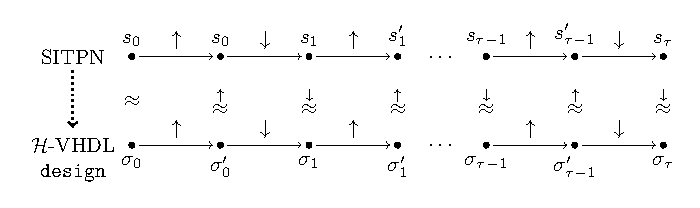
\includegraphics[keepaspectratio,width=\textwidth]{trace-comparison-full.eps}
  \caption{Comparison between the execution trace of a SITPN model (on
    the upper part) and the execution trace of the \hvhdl{} design
    resulting from the HM2T (on the lower part).}
  \label{fig:trace-comparison}
\end{figure}

In Figure~\ref{fig:trace-comparison}, $\tau$ indicates an arbitrary
number of clock cycles. To perform the proof of semantic preservation,
we must prove that every pair of states considered at the same time
point are similar w.r.t. to our own similarity relation.  Let us
introduce our general similarity criterions between a SITPN state and
a \hvhdl{} state through the relation presented in
Definition~\ref{def:state-sim}.

\begin{definition}[State similarity relation]
  \label{def:state-sim}
  For a given $sitpn\in{}SITPN$, a \hvhdl{} design $d\in{}design$, and
  a binder $\gamma\in{}WM(sitpn,d)$, an SITPN state $s\in{}S(sitpn)$
  and a design state $\sigma\in\Sigma$ are similar, written
  $\gamma\vdash{}s\approx\sigma$ if
  \begin{enumerate}
  \item\label{item:sim-mark} $\forall{}p\in{}P,$
    $~s.M(p)=\sigma(\gamma(p))($\texttt{s\_marking}$)$.
  \item\label{item:sim-tc}
    $\forall{}t\in{}T_i,$\\
    $\big(u(I_s(t))=\infty\land{}s.I(t)\le{}l(I_s(t))\Rightarrow{}s.I(t)=\sigma(\gamma(t))($\texttt{s\_time\_counter}$)\big)$\\
    $\land\big(u(I_s(t))=\infty\land{}s.I(t)>{}l(I_s(t))\Rightarrow{}\sigma(\gamma(t))($\texttt{s\_time\_counter}$)=l(I_s(t))\big)$\\
    $\land\big(u(I_s(t))\neq\infty\land{}s.I(t)>{}u(I_s(t))\Rightarrow{}\sigma(\gamma(t))($\texttt{s\_time\_counter}$)=u(I_s(t))\big)$\\
    $\land\big(u(I_s(t))\neq\infty\land{}s.I(t)\le{}u(I_s(t))\Rightarrow{}s.I(t)=\sigma(\gamma(t))($\texttt{s\_time\_counter}$)\big)$.
  \item\label{item:sim-reset} $\forall{}t\in{}T_i,$
    $s.reset_t(t)=\sigma(\gamma(t))($\texttt{s\_reinit\_time\_counter}$)$.
  \item\label{item:sim-cond}
    $\forall{}c\in\mathcal{C},~s.cond(c)=\sigma(\gamma(c))$.
  \item\label{item:sim-act}
    $\forall{}a\in\mathcal{A},~s.ex(a)=\sigma(\gamma(a))$.
  \item\label{item:sim-fun}
    $\forall{}f\in\mathcal{F},~s.ex(f)=\sigma(\gamma(f))$.
  \end{enumerate}
\end{definition}

In Definition~\ref{def:state-sim}, the binder structure $\gamma$ that
is generated by the HM2T relates the elements of the SITPN model to
the elements of the \hvhdl{} design, and thus enables the comparison
between a SITPN state and a \hvhdl{} state. In
Definition~\ref{def:state-sim}, Point~\ref{item:sim-mark} relates the
marking value of a place $p$ at state $s$ to the value of the
\texttt{s\_marking} signal, which is an internal signal of the PDI
identified by $\gamma(p)$. Here, the expression $\sigma(\gamma(p))$
returns the internal state of a PDI by looking up the component store
of state $\sigma$. Points~\ref{item:sim-tc} and \ref{item:sim-reset}
similarly relate the value of time counters (resp. reset orders) of
transitions to the value of the signals $\texttt{s\_time\_counter}$
(resp. $\texttt{s\_reinit\_time\_counter}$) in the internal state of
the corresponding TDIs. In Point~\ref{item:sim-cond}
(resp. \ref{item:sim-act} and \ref{item:sim-fun}), the Boolean value
of conditions (resp. actions and functions) are compared to the value
of input (resp. output) ports of the output design, also based on the
$\gamma$ binder.  As one can observe in Point~\ref{item:sim-tc}, due
to the specific implementation of time intervals with an infinite
upper bound in \hvhdl{}, the relation between the value of a time
counter and the value of the $\texttt{s\_time\_counter}$ signal can
not be restricted to a simple equality.

As shown in Figure~\ref{fig:trace-comparison}, we make a distinction
between the state similarity after a rising edge phase and after a
falling edge phase. The definitions of the post rising edge similarity
relation, written $\stackrel{\uparrow}{\approx}$, and the post falling
edge similarity relation, written $\stackrel{\uparrow}{\approx}$, are
restrictions of the general definition. After a rising edge phase, the
equality between the value of conditions and the value of condition
ports (i.e. Point~\ref{item:sim-cond} of
Definition~\ref{def:state-sim}) does not hold. And after a falling
edge phase, the equality between the value of time counter reset
orders and the value of the \texttt{srtc} signals
(i.e. Point~\ref{item:sim-reset} of Definition~\ref{def:state-sim})
does not hold. However, these divergences do not impact the
computation logic of the overall so that to create further behavioral
divergences between the input SITPN model and the output \hvhdl{}
design.


%%% Local Variables:
%%% mode: latex
%%% TeX-master: "main"
%%% End:

\include{concl}

\begin{appendices}

  \section{The place design in abstract \hvhdl{} syntax}
\label{app:place-design}

\begin{lstlisting}[language=VHDL,
  label={lst:place-design-abss},
  caption={The \texttt{place} design in \hvhdl{} abstract syntax.},
  basicstyle=\fontsize{8}{10}\selectfont,
  framexleftmargin=1.5em,
  xleftmargin=2em,
  numbers=left,
  numberstyle=\tiny\ttfamily]
{
    
-- Generic constant declarations
$gens$={
  (input_arcs_number, nat(0,NATMAX), 1), 
  (output_arcs_number, nat(0,NATMAX), 1),
  (maximal_marking, nat(0,NATMAX), 1)},

-- Port declarations
$ports=${
  (in, initial_marking, nat(0, maximal_marking)),
  (in, input_arcs_weights, array (nat(0, 255), 0, sub(input_arcs_number, 1))),
  (in, output_arcs_types, array (nat(0, 2), 0, sub(output_arcs_number, 1))),
  (in, output_arcs_weights, array (nat(0, 2), 0, sub(output_arcs_number, 1))),
  (in, input_transitions_fired, array (bool, 0, sub(input_arcs_number, 1))),          
  (in, output_transitions_fired, array (bool, 0, sub(output_arcs_number, 1))),
  (out, output_arcs_valid, array (bool, 0, sub(output_arcs_number, 1))),
  (out, priority_authorizations, array (bool, 0, sub(output_arcs_number, 1))),
  (out, reinit_transitions_time, array (bool, 0, sub(output_arcs_number, 1))),
  (out, marked, bool)},
  
-- Internal signal declarations
$sigs$={(s_input_tokens_sum, nat(0, maximal_marking)),
        (s_marking, nat(0, maximal_marking)),
        (s_output_tokens_sum, nat(0, maximal_marking))},
       
-- Behavior  
$beh$=
ps (input_tokens_sum, 
  {(v_tokens_sum, nat(0, maximal_marking))},
  v_tokens_sum := 0;
  for (i, 0, sub(input_arcs_number, 1)){
     if (input_transitions_fired(i)) { 
        v_tokens_sum := add(v_tokens_sum, input_arcs_weights(i))
     } else { null }
  };
  s_input_tokens_sum <= v_tokens_sum)
$\vert\vert$
ps (output_tokens_sum, 
  {(v_tokens_sum, nat(0, maximal_marking))},
  v_tokens_sum := 0;
  for (i, 0, sub(output_arcs_number, 1)) {
    if (and(output_transitions_fired(i), eq(output_arcs_types(i), 0))) {
      v_tokens_sum := add(v_tokens_sum, output_arcs_weights(i))
    } else { null }
  };
  s_output_tokens_sum <= v_tokens_sum)
$\vert\vert$    
ps (marking, $\emptyset$,
  rst { s_marking <= initial_marking }
  else {
    rising {
      s_marking <= add(s_marking, sub(s_input_tokens_sum, s_output_tokens_sum))
    }
  })
$\vert\vert$
ps (determine_marked, $\emptyset$, marked <= gt(s_marking, 0))
$\vert\vert$  
ps (marking_validation_evaluation, $\emptyset$,
  for (i, 0, sub(output_arcs_number, 1)) {
    output_arcs_valid(i) <= 
    or(and(or(eq(output_arcs_types(i), 0),
              eq(output_arcs_types(i), 1)),
           ge(s_marking, output_arcs_weights(i))),
       and(eq(output_arcs_types(i), 2),
           lt(s_marking, output_arcs_weights(i))))
  })
$\vert\vert$
ps (priority_evaluation, 
  {(v_saved_output_tokens_sum, nat(0, maximal_marking))},
  v_saved_output_tokens_sum := 0;
  for (i, 0, sub(output_arcs_number, 1)) {
    priority_authorizations(i) <= ge(s_marking, add(v_saved_output_tokens_sum, output_arcs_weights(i));
    if (and(output_transitions_fired(i), eq(output_arcs_types(i), 0))) {
      v_saved_output_tokens_sum := add(v_saved_output_tokens_sum, output_arcs_weights(i))
    } else { null }
  })
$\vert\vert$      
ps (reinit_transitions_time_evaluation, $\emptyset$,
  rst { 
    for (i, 0, sub(output_arcs_number, 1)) {
      reinit_transitions_time(i) <= false
    }
  } else {
    rising {
      for (i, 0, sub(output_arcs_number, 1)) {
        reinit_transitions_time(i) <=
        or(and(and(or(eq(output_arcs_types(i), 0),
                      eq(output_arcs_types(i), 1)),
                   lt(sub(s_marking, s_output_tokens_sum),
                      output_arcs_weights(i)))
               gt(s_output_tokens_sum, 0)),
               output_transitions_fired(i))
      }
    }
  })
}
\end{lstlisting}

%%% Local Variables:
%%% mode: latex
%%% TeX-master: "main"
%%% End:

  \section{The transition design in abstract \hvhdl{} syntax}
\label{app:trans-design}

\begin{lstlisting}[language=VHDL,
label={lst:trans-design-abss},
caption={The \texttt{transition} design in \hvhdl{} abstract syntax.},
framexleftmargin=1.5em,
xleftmargin=2em,
numbers=left,
numberstyle=\tiny\ttfamily,
basicstyle=\fontsize{8}{10}\selectfont]
{

-- Generic constant declarations
$gens$={
  (transition_type, nat(0, 3), 0),
  (input_arcs_number, nat(0, NATMAX), 1),
  (conditions_number, nat(0, NATMAX), 1),
  (maximal_time_counter, nat(0, NATMAX), 1)},

-- Port declarations
$ports$={
  (in, input_conditions, array(bool, 0, sub(conditions_number, 1)),
  (in, time_A_value, nat(0, maximal_time_counter)),
  (in, time_B_value, nat(0, maximal_time_counter)),
  (in, input_arcs_valid, array(bool, 0, sub(input_arcs_number, 1))),
  (in, reinit_time, array(bool, 0, sub(input_arcs_number, 1))),
  (in, priority_authorizations, array(boolean, 0, sub(input_arcs_number, 1))),
  (out, fired, bool)},

-- Internal signal declarations
$sigs$={
  (s_condition_combination, bool),
  (s_enabled, bool),
  (s_firable, bool),
  (s_firing, bool),
  (s_priority, bool),
  (s_reinit, bool),
  (s_time_counter, nat(0, maximal_time_counter)},

-- Behavior
$beh$=
ps (condition_evaluation, {(v_internal_condition, bool)},
  v_internal_condition := true;
  for (i, 0, sub(conditions_number, 1)) {
    v_internal_condition := and(v_internal_condition, input_conditions(i))
  };
  s_condition_combination <= v_internal_condition)
$\vert\vert$
ps (enable_evaluation, {(v_internal_enabled, bool)},
  v_internal_enabled := true;
  for (i, 0, sub(input_arcs_number, 1)) {
    v_internal_enabled := and(v_internal_enabled, input_arcs_valid(i))
  };
  s_enabled <= v_internal_enabled)
$\vert\vert$
ps (reinit_time_counter_evaluation, {(v_internal_reinit_time_counter, bool)},
  v_internal_reinit_time_counter := false;
  for (i, 0, sub(input_arcs_number, 1)) {
    v_internal_reinit_time_counter := or(v_internal_reinit_time_counter, reinit_time(i))
  };
  s_reinit_time_counter <= v_internal_reinit_time_counter)
$\vert\vert$
ps (time_counter, $\emptyset$,
  rst { s_time_counter <= 0 }
  else {
    falling {
      if (and(s_enabled, neq(transition_type, 0))) {
        if (eq(s_reinit_time_counter, false)) {
          if (s_time_counter < maximal_time_counter) {
            s_time_counter <= s_time_counter + 1
          } else { null }
        }
        else { s_time_counter <= 1 }
      }
      else { s_time_counter <= 0 }
    }
  })
$\vert\vert$
ps (firing_condition_evaluation, $\emptyset$, 
  s_firing_condition <= 
  s_condition_combination
  and s_enabled
  and (eq(transition_type, 0)
       or (eq(s_reinit_time_counter, false) 
           and ((eq(transition_type, 1) 
                 and ge(s_time_counter, sub(time_A_value, 1)) 
                 and (s_time_counter < time_B_value))
               or (eq(transition_type, 2) 
                   and eq(s_time_counter, sub(time_A_value, 1)))
               or (eq(transition_type, 3) 
                   and ge(s_time_counter, sub(time_A_value, 1)))))                              
       or (s_reinit_time_counter
           and neq(transition_type, 0)
           and eq(time_A_value, 1))))
$\vert\vert$
ps (priority_authorization_evaluation, {(v_priority_combination, bool)},
  v_priority_combination := true;
  for (i, 0, sub(input_arcs_number, 1)) {
    v_priority_combination := and(v_priority_combination, priority_authorizations(i))
  };
  s_priority_combination <= v_priority_combination)
$\vert\vert$
ps (firable, $\emptyset$,
  rst { s_firable <= false }
  else { falling { s_firable <= s_firing_condition } })
$\vert\vert$
ps (fired_evaluation, $\emptyset$, fired <= and(s_firable, s_priority_combination))
\end{lstlisting}

%%% Local Variables:
%%% mode: latex
%%% TeX-master: "main"
%%% End:

  \section{Generic constant and signal names reference}
\label{sec:cnsts-sigs-names}

\begin{table}[h]
  \resizebox{\textwidth}{!}{%
  \begin{tabular}{|c|c|c|c|}
    \hline
    \multicolumn{4}{|c|}{\textbf{Generic constants and signals reference}} \\
    \hline
    \textit{Full name} & \textit{Alias} & \textit{Category} & \textit{Type} \\
    \hline
    \texttt{input\_arcs\_number} & \texttt{ian} & generic constant (T) & $\mathtt{nat}(0,\mathtt{NATMAX})$ \\
    \hline
    \texttt{transition\_type} & \texttt{tt} & generic constant (T) & $\{\mathtt{not\_temp},\mathtt{temp\_a\_b},$ \\
                       & & & $\mathtt{temp\_a\_a},\mathtt{temp\_a\_inf}\}$ \\
    \hline
    \texttt{conditions\_number} & \texttt{cn} & generic constant (T) & $\mathtt{nat}(0,\mathtt{NATMAX})$ \\
    \hline
    \texttt{maximal\_time\_counter} & \texttt{mtc} & generic constant (T) & $\mathtt{nat}(0,\mathtt{NATMAX})$ \\
    \hline
    \texttt{time\_A\_value} & \texttt{A} & input port (T) & $\mathtt{nat}(0,\mathtt{mtc})$ \\
    \hline
    \texttt{time\_B\_value} & \texttt{B} & input port (T) & $\mathtt{nat}(0,\mathtt{mtc})$ \\
    \hline
    \texttt{input\_conditions} & \texttt{ic} & input port (T) & $\mathtt{array(\mathtt{bool},0,\mathtt{cn}-1)}$ \\
    \hline
    \texttt{reinit\_time} & \texttt{rt} & input port (T) & $\mathtt{array}(\mathtt{bool},0,\mathtt{ian}-1)$ \\
    \hline
    \texttt{input\_arcs\_valid} & \texttt{iav} & input port (T) & $\mathtt{array}(\mathtt{bool},0,\mathtt{ian}-1)$ \\
    \hline
    \texttt{priority\_authorizations} & \texttt{pauths} & input port (T) & $\mathtt{array}(\mathtt{bool},0,\mathtt{ian}-1)$ \\
    \hline
    \texttt{fired} & \texttt{f} & output port (T) & $\mathtt{bool}$ \\
    \hline
    \texttt{s\_condition\_combination} & \texttt{scc} & internal signal (T) & $\mathtt{bool}$ \\
    \hline
    \texttt{s\_reinit\_time\_counter} & \texttt{srtc} & internal signal (T) & $\mathtt{bool}$ \\
    \hline
    \texttt{s\_priority\_combination} & \texttt{spc} & internal signal (T) & $\mathtt{bool}$ \\
    \hline
    \texttt{s\_firable} & \texttt{sfa} & internal signal (T) & $\mathtt{bool}$ \\
    \hline
    \texttt{s\_enabled} & \texttt{se} & internal signal (T) & $\mathtt{bool}$ \\
    \hline
    \texttt{s\_time\_counter} & \texttt{stc} & internal signal (T) & $\mathtt{nat}(0,\mathtt{mtc})$ \\
    \hline
    \texttt{s\_firing\_condition} & \texttt{sfc} & internal signal (T) & $\mathtt{bool}$ \\
    \hline
    \hline
    \texttt{input\_arcs\_number} & \texttt{ian} & generic constant (P) & $\mathtt{nat}(0,\mathtt{NATMAX})$ \\
    \hline
    \texttt{output\_arcs\_number} & \texttt{oan} & generic constant (P) & $\mathtt{nat}(0,\mathtt{NATMAX})$ \\
    \hline
    \texttt{maximal\_marking} & \texttt{mm} & generic constant (P) & $\mathtt{nat}(0,\mathtt{NATMAX})$ \\
    \hline
    \texttt{initial\_marking} & \texttt{im} & input port (P) & $\mathtt{nat}(0,\mathtt{mm})$ \\
    \hline
    \texttt{output\_arcs\_types} & \texttt{oat} & input port (P) & $\mathtt{array}(\{\mathtt{basic},\mathtt{test},\mathtt{inhib}\}, 0, \mathtt{oan}-1)$ \\
    \hline
    \texttt{output\_arcs\_weights} & \texttt{oaw} & input port (P) & $\mathtt{array}(\mathtt{nat}(0,255),0,\mathtt{oan}-1)$ \\
    \hline
    \texttt{output\_transitions\_fired} & \texttt{otf} & input port (P) & $\mathtt{array}(\mathtt{bool},0,\mathtt{oan}-1)$ \\
    \hline
    \texttt{input\_arcs\_weights} & \texttt{iaw} & input port (P) & $\mathtt{array}(\mathtt{nat}(0,255),0,\mathtt{ian}-1)$ \\
    \hline
    \texttt{input\_transitions\_fired} & \texttt{itf} & input port (P) & $\mathtt{array}(\mathtt{bool},0,\mathtt{ian}-1)$ \\
    \hline
    \texttt{output\_arcs\_valid} & \texttt{oav} & output port (P) & $\mathtt{array}(\mathtt{bool},0,\mathtt{oan}-1)$ \\
    \hline
    \texttt{reinit\_transitions\_time} & \texttt{rtt} & output port (P) & $\mathtt{array}(\mathtt{bool},0,\mathtt{oan}-1)$ \\
    \hline
    \texttt{priority\_authorizations} & \texttt{pauths} & output port (P) & $\mathtt{array}(\mathtt{bool},0,\mathtt{oan}-1)$ \\
    \hline
    \texttt{marked} & \texttt{m} & output port (P) & $\mathtt{bool}$ \\
    \hline
    \texttt{s\_marking} & \texttt{sm} & internal signal (P) & $\mathtt{nat}(0,\mathtt{mm})$ \\
    \hline
    \texttt{s\_output\_token\_sum} & \texttt{sots} & internal signal (P) & $\mathtt{nat}(0,\mathtt{mm})$ \\
    \hline
    \texttt{s\_input\_token\_sum} & \texttt{sits} & internal signal (P) & $\mathtt{nat}(0,\mathtt{mm})$ \\
    \hline
  \end{tabular}}
  \caption[Constants and signals reference for the \hvhdl{}
  \texttt{transition} and \texttt{place} designs.]{Constants and
    signals reference for the \hvhdl{} transition and place
    designs. In the \textit{Category} column, T (resp. P) indicates a
    generic constant, input port, output port or internal signal
    defined in the \texttt{transition} (resp. \texttt{place})
    design. }
  \label{tab:consts-and-sigs-ref}
\end{table}



%%% Local Variables:
%%% mode: latex
%%% TeX-master: "main"
%%% End:

\end{appendices}


\bibliography{references}

\end{document}
